\documentclass[11pt,letterpaper]{article}
\usepackage[T1]{fontenc}
\usepackage{lmodern}
\usepackage[margin=0.95in]{geometry}
\usepackage{amsmath}
\usepackage{booktabs}
\usepackage{graphicx}
\usepackage[numbers,sort&compress]{natbib}
\usepackage{xurl}
\usepackage[hidelinks]{hyperref}
\hypersetup{
  pdftitle={When a Language Model Server Reports a Different Token},
  pdfauthor={Yufeiyang Chen},
  pdfkeywords={test oracles, language model serving, API testing, token log probabilities, reinforcement learning}
}
\urlstyle{same}
\newcommand{\doi}[1]{\href{https://doi.org/#1}{doi:\,#1}}
\title{When a Language Model Server Reports a Different Token}
\author{Yufeiyang Chen}
\date{November 18, 2026}

\begin{document}
\maketitle
\begin{abstract}
Applications use the probability attached to a generated token to score answers and update policies. Does the reported probability belong to the token the model sampled? We test the formatter on the same sampling event with the list of alternatives enabled and suppressed. On two live MLX-LM releases, asking for alternatives caused the first alternative to replace the sampled token in the metadata. A release census locates the regression across eight consecutive versions. On 64 public prompts, 528 of 1,488 positions named the wrong token. Five alternatives omitted the sampled token at 204 positions. We show why even a client given the true IDs cannot always recover which answer had the highest score. On 80 fresh four-answer groups, a seeded replay issued 76 rankings, all matching the original sampled-score rankings. Four repeated requests passed the matching checks despite returning different score sequences. On 2,108 held-out science questions, ranking the same answers by the sampled scores and by the reported scores selected different texts on 846 questions. Correctness changed in both directions. A controlled online sentiment learner lost 1.90 percentage points of expected correctness across 128 training seeds. A second workload confirmed changes to actual decoder updates but did not establish a performance loss. The artifact includes a source patch, a regression test without model weights, and paired observations that distinguish score substitution from other token-reporting failures.

\end{abstract}

\section{Introduction}
A server generated the phrase \emph{In the realm of monumental grandeur}. At the fifth output position it sampled the vocabulary entry for a leading space followed by \emph{monumental}, ID 24313. The decoder assigned it a log probability of $-4.4375$. The response metadata for the same position named \emph{architecture}, ID 6277, with a log probability of $-2.25$. Both words fit the context. Both numbers are plausible. The generated text contains the right word. All five alternatives omit its score.

This example comes from an ordinary chat request to a released language model server. The user requested the probabilities of five alternatives alongside the response. Adding that information should preserve the identity of the token that was generated. The distinction matters whenever an application reads the probability as evidence about the text. An evaluator that averages the reported scores can make an answer look more likely than it was. A policy optimizer that pairs an action with the wrong old probability can change its gradient even if a verifier correctly scored the answer.

Testing the correspondence presents two difficulties. A second request can legitimately generate different tokens. Even when its final text agrees, the sampled IDs or their scores can differ. We record the native emission and give the released response formatter the same event twice, changing only the presence of the alternatives. This allows a test to reject a wrong attribution without predicting the next word. We then ask what remains recoverable once the original sampling event is gone.

The risk was visible in practice before this study. The public INDRA scoring pipeline enforces greedy decoding for in-call probabilities and warns that a reported token stream can diverge from sampled text at positive temperature~\cite{indra}. That observation poses an engineering question. Can one pinpoint when the record becomes wrong, detect the error without a sampler-side observation, and show which downstream decisions actually depend on it?

We ask three questions. \emph{RQ1} localizes token substitution in a released server and distinguishes it from omitted positions and damaged token bytes in independent implementations. \emph{RQ2} compares client remedies under four information conditions: an archived response, supplied token IDs, a second seeded request, and access to the original generation. \emph{RQ3} follows the affected fields into a released evaluator, answer selection with external labels, and controlled online learning.

\section{The contract at the serving boundary}
Let $u_t$ denote the ID emitted at position $t$, $s_t$ the score the decoder passes to the serializer for $u_t$, and $A_{t,k}$ the supplied list of up to $k$ alternatives. An interface can expose the sampled ID directly, or identify the selected token by a vocabulary string or bytes. In the MLX interface under test, the candidate-enabled representation has an integer ID, a vocabulary string, and a log probability per position. The candidate-disabled representation exposes ID and score. The selected pair in both must refer to $(u_t,s_t)$. The API contract distinguishes output tokens from alternatives. For example, vLLM documents that its logprob mapping includes the chosen token even if it falls outside the requested top set~\cite{openai,vllm}. The Chat Completions schema allows unavailable bytes and a sentinel for a sufficiently low score~\cite{chatschema}. Checks on numeric or byte equality must respect those conventions. The names and encodings of fields can differ across APIs. The invariant concerns the identity each field represents.

The score also has a stage. In the MLX chat experiments $s_t$ is the raw model log probability indexed by $u_t$, before temperature sampling. Temperature can change how often the engine selects a token. It does not change which entry in the raw score vector belongs to that token. In the two-action training experiment we instead need the old probability under the restricted behavior distribution. There we have both allowed actions' scores and normalize them on identical support in every arm.

A simpler property is available when the native emission cannot be observed. Decode the sequence of reported IDs with the engine's tokenizer and compare it with the transcript under the same rendering rules. This gives a response-level alarm. It generally gives neither a unique inverse from text to IDs nor the missing scores. Suppose an emitted ID is absent from a top-five list. Even for normalized probabilities, the list constrains only the total remaining mass and the cutoff. Two unlisted tokens can exchange sufficiently small amounts of mass without changing the list. Knowing which one was sampled leaves its individual score undetermined by these fields. A consumer with the exact model state could recompute the distribution. Our candidate-only baseline has no such access.

\section{Study design}
\subsection{What the oracle observes}
A read-only observation at the generator iterator passed to the HTTP handler saves each yielded position's selected ID and raw score. A second observation at the native serializer saves the IDs and scores the handler supplies. We join these records to the non-streaming chat response by request and position, check lengths against usage, and retain terminal positions when the server counts them. Re-tokenization is a competing client method. It supplies no ground truth.

We send the same prompt and seed with no alternatives requested, then with one or five. We check whether the emitted sequences match across requests. To remove any dependence on repeatable sampling, we also invoke the original serializer on identical captured arguments with the candidate list present or suppressed. This holds weights, logits, and the sampling event fixed. A failure specific to the candidate-enabled path then localizes the error after the sampled pair reached the serializer. A separate intervention changes just the selected fields after the original serializer returns. Comparing the entire response object after substituting those fields tests whether the transcript, finish reason, usage, request identity or alternatives changed.

\subsection{Workloads and units}
The initial clue arose during a restricted two-action learning experiment. We exclude those traces from the ordinary-chat workload. The localization suite fixes twelve fresh prompts before generation. They cover translation, short explanations, structured output, code completion, and open continuation. Each prompt receives a fixed seed shared across its three requests. We run released MLX-LM 0.31.3 with its stock sampler and, separately, an eager categorical sampler as a control for reported worker random-state behavior~\cite{mlxseed}. We repeat the stock experiment with matching 0.32.2 MLX-LM, MLX and Metal release wheels~\cite{mlx}. Each uses SmolLM2-135M-Instruct~\cite{smol}, unrestricted vocabulary, temperature 0.8, $p=1$, and a limit of 12 positions. The number of reported alternatives is distinct from a top-$k$ sampling filter.

We next select prompts from the public IFEval collection~\cite{ifeval}. Before retrieving their text or observing outcomes, the protocol specifies ranking all 541 stable integer keys by the SHA-256 digest of a fixed prefix and the decimal key. We take the first 64. The research artifact records the ranking digests, selected prompt hashes, and source revision. We send each original user prompt once to the newer release, requesting five alternatives at temperature 0.8 with a 24-position cap. Each request yields the original response object captured inside the server before correction and the corrected response delivered over HTTP. In the twelve-prompt experiment the original response itself traverses HTTP. Sixty public-prompt responses reached 24 positions. The other four contributed 18, 18, 9, and 3 positions.

We report the finite workload in full. A position-weighted proportion describes the volume of wrong metadata. An unweighted per-response distribution describes what clients encountered. Counting positions as independent replicates would produce spurious precision. The independent engine experiment uses a separate implementation and probability reference. In the fixed-trace study the unit is one of three distinct trajectories. In the online intervention it is a paired training seed. We keep earlier aborted setup attempts separate: an incompatible optional observer field changed in the new MLX release, the initial repair wrapper lacked the full call signature, and the first public-prompt launch preceded acquisition of the pinned data. We analyze the complete runs following those setup fixes, using each condition once.

\subsection{AI assistance and provenance}
OpenAI Codex agents specified the input selection and comparison rules, implemented the instrumentation and replays, ran the serving and downstream experiments, inspected source and trace records, computed the tables and empirical distribution plot, and drafted the text. GPT-6.2 Sol agents in Codex prepared the independent-engine experiments, designed and ran the online learning intervention, and built checks on saved observations. The coordinating agent designed the answer-ranking experiments, inspected the primary records, and integrated the comparisons. Gemini in Antigravity contributed to earlier reward-pipeline explorations. Those explorations supply no observations in the denominators here. Agents also designed and ran the recovery, cache-order, judge, decoder-update and calibration experiments, prepared the release patch, and independently checked tie rules, precision and artifact replays. The oracle compares executable outputs and recorded IDs. Agreement between agents supplies no independent labels.

\section{RQ1. What changes when alternatives are requested?}
\subsection{A substitution in two released serializers}
Table~\ref{tab:release} shows the twelve-prompt localization results. Within each row, all twelve complete sampled sequences were identical across the three request settings. The serializer passed the sampled ID and raw score correctly when alternatives were absent in every condition. At widths one and five, the same output positions had wrong IDs within each condition. Replaying the identical serializer inputs with the list suppressed restored the pair. The eager sampler changed which tokens the model emitted, yet it left the field substitution intact. The newer release exhibited the same mechanism with its matching runtime.

\begin{table}[htbp]
\centering
\caption{Same twelve prompts per condition, 144 generated positions per width. Each triple gives the number of wrong IDs with alternatives omitted, one requested, and five requested. The last three columns refer to width five.}
\label{tab:release}
\begin{tabular}{@{}lcrrr@{}}\toprule
MLX-LM and sampler & Wrong IDs & Wrong scores & Sample outside five & Prompts affected\\\midrule
0.31.3 stock & 0 / 44 / 44 & 44 & 17 & 12/12\\
0.31.3 eager & 0 / 36 / 36 & 35 & 12 & 11/12\\
0.32.2 stock & 0 / 45 / 45 & 42 & 17 & 11/12\\\bottomrule
\end{tabular}
\end{table}

The cause is visible in \texttt{APIHandler.generate\_response}. With no candidates, the function takes the selected ID and probability from the two sequences passed by the caller. With candidates, it builds each outer entry by copying the first element of that position's candidate list and appending the full list. The list is produced by partitioning the probability vector. Its first element is an alternative and need not be the global maximum. Treating it as the sample happens to work whenever its ID equals the draw. A greedy-only test or a fixture with one overwhelmingly likely token can therefore miss the defect. A numeric-only comparison also misses wrong identities with tied scores.

On the 64 public prompts, every response had at least one substitution. Of 1,488 positions, 528 (35.5\%) named a different ID and 521 supplied a different raw score. Seven substitutions paired different IDs with equal scores. In 324 of the substitutions the sampled ID appeared elsewhere among the alternatives. In the remaining 204 it was absent. The median within-response error fraction was 37.5\%, ranging from 5.6\% to 70.8\% (Figure~\ref{fig:prompt}). These rates describe this checkpoint, API path, display width, temperature, and workload. The results establish one mechanism across two software releases.

\paragraph{Holding out the model.}
Would the same serializer fail with a different architecture and tokenizer? We fixed the first twelve prompts in the existing IFEval panel and used the released four-bit Qwen2.5-0.5B-Instruct checkpoint with its own tokenizer~\cite{qwen}. For each prompt we sent three HTTP requests to MLX-LM 0.32.2 with the same seed. We omitted alternatives in the first, requested five in the second, and requested five with the local repair in the third. Each used stock sampling, temperature 0.8, and a 24-position limit. We also retained the native, pre-serialization and no-list views of the same draw. This is an independent checkpoint on deliberately overlapping prompts.

All twelve output ID sequences, raw scores and message contents matched across the three requests within each prompt. Each arm yielded 262 positions (ten answers of length 24, one of 14, and one of eight). The unmodified five-candidate response misidentified 117/262 tokens and their scores, affecting 11/12 answers. The first listed ID occupied every outer entry. The true ID was absent from 54/262 lists, so even ID-assisted lookup recovered only 208 scores. The omitted-list and repaired HTTP arms had zero ID or score errors. The repaired response preserved all fields outside the three selected-token values relative to its own original serialization. This model holdout tests a second architecture and tokenizer. It provides no population prevalence estimate across checkpoints.

\subsection{How decoding exposes the fault}
Greedy decoding can conceal a substitution that is deterministic inside the formatter. We excluded the original 64 IFEval prompts, ranked the remaining keys by a newly fixed hash and used the first 40. With the same SmolLM2 checkpoint, five returned alternatives and the 24-token cap, we generated once greedily and four times per prompt at each positive temperature. Each request preserved both the original HTTP object and a separate record of the sampled pairs. All 12,039 outer pairs matched the first returned candidate. The candidate-free projection of the same draw matched the sampled pair throughout. The formatter obtains its five candidates by partial selection, so its contract does not require ordering the five entries by score. The empirical agreement here is with the first entry as returned.

\begin{table}[htbp]
\centering
\caption{Decoding on the same 40 new questions. Last column counts prompts where ranking four answers by the reported mean log probability selected different text than ranking them by the native mean.}
\label{tab:temperature}
\begin{tabular}{@{}rrrrrr@{}}\toprule
Temperature & Draws & Positions & Wrong ID & ID outside five & Changed text /40\\\midrule
0 & 40 & 928 & 0 & 0 & ---\\
0.4 & 160 & 3,720 & 573 & 49 & 6\\
0.8 & 160 & 3,641 & 1,240 & 442 & 14\\
1.2 & 160 & 3,750 & 2,514 & 1,889 & 12\\\bottomrule
\end{tabular}
\end{table}

Table~\ref{tab:temperature} shows when the error becomes observable. Greedy generation always selected the first candidate on this panel. At temperature 0.8 the ID error frequency was 34.1\%, close to the original 35.5\% on disjoint prompts. At 1.2 it reached 67.0\%. The unit for comparing final choices is a question, with the same four draws supplied to both ranking rules. Thus a larger fraction of misreported positions need not cause more questions to change winners. The paired comparisons concern the entire output, which can change with temperature.

\paragraph{Later positions in naturally terminating answers.}
We drew 36 unused IFEval prompts by a fixed hash. At temperature 0.8 we increased the cap to 512 tokens. Five responses reached the cap and 31 stopped naturally. At positions 1--24, 318 of 847 IDs differed. The counts were 752/2,109 at 25--96, 1,051/3,225 at 97--256 and 594/2,170 at 257--512. The same-event candidate-free records agreed at all 8,351 positions. Among the 26 responses reaching token 97, the prespecified within-response change from the first band to positions 97--256 was $-4.69$ percentage points (95\% prompt bootstrap $[-13.04,3.10]$). The defect persists into long answers. The paired interval leaves the depth trend unresolved.

\subsection{Tracing the change across published versions}
We reduced the opening example to a single sampled position suitable for a CPU-only regression test. We pass its selected ID, score, and five original alternatives to the released serializer method with a minimal non-streaming handler state. A second position from the same response serves as a chance-agreement control: the sampler actually chose the first candidate there. The test executes the unmodified method body without model weights, Metal, or HTTP. It fails when the candidate-visible pair changes, even if the five alternatives themselves are intact. Wrapping either of the two live-tested methods with the repair makes both cases pass.

We froze the inputs and release interval before testing additional versions. We included every non-yanked final PyPI release from 0.30.0 through 0.32.2, spanning the preceding minor line and both live-tested releases. We verified all twelve wheels against their published SHA-256 digests and extracted six distinct serializer bodies. Four releases, ending at 0.30.5, reported the sampled pair in parallel arrays and returned the correct values on both cases. The next eight releases, beginning with 0.30.6, produced per-position objects and all substituted the first candidate on the outside-list case. Every version preserved the selected pair when the candidates were suppressed and passed the first-candidate control. No release in the interval had an unresolved result.

The corresponding upstream change, merged on February 3, 2026, replaced the parallel arrays with the new chat response format and introduced the copy of the first candidate~\cite{change}. The first affected wheel in the interval was published on February 4, and the eighth on October 16. This result dates one regression in public software. The number of releases provides neither a count of distinct defects nor a count of affected installations.

\subsection{An independent engine separates substitution from omission}
We repeated the test on the first twelve public prompts in their already frozen order with an independent implementation, llama.cpp~\cite{llama}. This holds out an engine, reusing prompts deliberately. We used the official macOS binary b12359, commit \texttt{b1b770d9}, and an F16 GGUF conversion of the same checkpoint. The native non-streaming completion API received the engine's templated prompt IDs, a fixed seed, temperature 0.8, and a 24-position limit. The native sampler settings and score-disabled response format differ from MLX. We made three calls per prompt, requesting zero, one, or five probabilities. A native array contains the selected IDs independently of probability-row construction. In a second process, we fed those IDs in order into libllama, took the full logits vector at each prefix, and computed the raw log-softmax at the selected ID. This shares the engine's model kernels but bypasses its sampling and probability formatting. We fixed a tolerance of 0.002 nats before running the test.

All twelve native ID sequences agreed across widths, for 280 sampled positions per setting. The zero-width response correctly omitted probability metadata. Both positive widths emitted 277 probability rows. Their selected IDs matched the native array under a unique ordered alignment. We independently reconstructed buffer completion from the native token bytes on the unequal-length response, verifying that alignment without consulting the reported IDs. All 277 scores agreed with the independent forward computation at each width, with maximum absolute discrepancy below 0.00027 nats. On those very rows, substituting the first candidate would have assigned the wrong ID at 89 of 277 positions. Giving a client the actual selected ID still left it without a score at 89 of 277 lists at width one and 18 at width five.

The three missing positions occurred in a single response (key 1582). Each contained the same two-byte prefix of a three-byte UTF-8 character. The engine saved the first sampled ID to its native array, buffered the incomplete bytes, then attached the complete character bytes to the probability row for the final byte. Three token IDs therefore had no corresponding row. Including those omissions, the five-candidate lookup abstained at 21/280 positions. A prior report by Kim describes this UTF-8 buffering mechanism in llama.cpp~\cite{murphy}. We independently reproduce that omission. The same engine preserves the selected ID on all aligned rows. A length check catches the incomplete response in llama.cpp and passes on all 64 affected MLX responses.

\subsection{A correct score can accompany damaged token bytes}
We tested the same 12 public prompts through a third inference engine, the published mistral.rs v0.9.5 server~\cite{mistralrs}. We observed its HTTP responses without instrumenting its Rust sampler. For stochastic generation we limited sampling to the four highest-scoring tokens, capped responses at eight positions, and reconstructed eligible token paths using an independent PyTorch forward pass and the visible response. We required a unique compatible path before judging identity or numeric error. In the width-five stochastic arm 11 of 12 responses admitted a unique witness (88 of 96 positions). The remaining response admitted multiple paths. We compared against the temperature-scaled full-vocabulary log-softmax before top-four truncation. All 88 reported scores agreed within the prespecified 0.02 nats (maximum error 0.00953). A first-candidate substitution would have misidentified 30 of those positions.

One ordinary Vietnamese response split each of two characters into two tokens. The first pair carried bytes \texttt{E1 BB} and \texttt{87} and the second \texttt{E1 BB} and \texttt{A5}. At all four positions the non-streaming API instead attached \texttt{EF BF BD}, the UTF-8 encoding of the replacement character. Three forced partial-byte controls reproduced the problem; three valid controls, including a token genuinely encoding the replacement character, retained the correct bytes. We then repeated all 12 stochastic requests with the same settings using streamed output. All 96 displayed token labels and reported scores matched the corresponding non-streaming records. The four differing byte arrays now contained the witnessed bytes. The mismatch concerns the byte field accompanying a selected score. We observed no evidence of assigning another token's score on the witnessed mistral.rs positions.

To test transfer beyond this one response, we fixed 12 hash-ranked parallel FLORES-200 devtest sentences and seven language strata before acquiring new outputs. For each prefix the server continued the text with ordinary top-four sampling, a fixed seed and a 16-token limit. Matching both transport modes yielded 84 paired responses and 1,336 aligned positions after excluding two streaming omissions of terminal EOS. All labels and scores agreed within the protocol tolerance. At 708 positions, non-streaming returned the replacement-character bytes for a piece of a completed character recoverable from the stream. These substitutions affected 359 completed characters across all 72 non-English responses (Vietnamese, Arabic, Hindi, Japanese, Chinese and Thai) and none of the 12 English responses. Script classification used the generated bytes, not just the language of the prompt. The strongest direct transport check reconstructs complete characters; 22 responses also had an incomplete trailing UTF-8 sequence at the generation limit, which we excluded from that count.

For the first two sentences in each language, independent PyTorch replay yielded unique compatible paths in 11 of the 14 cases. Of 176 witnessed positions, 85 non-streaming byte arrays and zero streamed arrays disagreed with the canonical bytes. Both modes retained the correct display labels and numeric scores within tolerance on all 176. Three responses with incomplete trailing bytes admitted no witness. These aligned translations share 12 source meanings and the language strata were chosen to probe byte boundaries; 72/84 is a property of that panel and model, not a traffic-weighted incidence estimate~\cite{flores}.

\subsection{Independent response builders}
We selected the latest stable vLLM and SGLang releases at the protocol freeze. A CPU harness executed their released non-streaming chat response builders on four shared synthetic sequences with known IDs, scores and ranks. They include a repeated ID, an emitted token outside the five most likely, and two distinct IDs with identical displayed text. Unlike the HTTP experiments, here the decoding inputs are constructed and the boundary is the formatter. We vary width among zero, one and five and compare ordinary token strings with the implementations' ID-bearing representations. Across 48 responses (72 position observations across settings), both builders preserved the selected scores and returned the expected row counts. All uniquely named selected tokens agreed. Plain-text identity was ambiguous in three of 18 positions per implementation; ID-bearing forms resolved the aliases. Deliberately substituting an ID and score, omitting a row, or changing only its score triggered the corresponding checks.

The alternative lists obey different rules. At width one, vLLM 0.34.0 allocated the slot to the selected ID in all six ID-mode positions, even when another token scored higher; at width five it also kept the selected ID in all six. SGLang 0.5.23 retained the actual outer pair while its separate candidate list contained the sampled ID at only two of six positions at width one and three at width five~\cite{vllm,sglangrel}. Thus rejecting every list that omits the sample would flag valid responses. The correct comparison is between the emission and the field claiming to describe it.

\section{RQ2. What can a client recover?}
We tested three levels of access on the 64 MLX responses. A transcript-only detector has the full response and the exact tokenizer. An ID-assisted client additionally has the true emitted IDs, as some native APIs supply. The producer already has both IDs and scores at the serializer input. We give each method the same five candidates. This comparison makes it possible to distinguish loss caused by rendering from loss caused by truncation of the candidate set.

\begin{table}[htbp]
\centering
\caption{Recovering selected ID--score pairs from 1,488 MLX positions. The first two methods abstain on a whole response if canonical token count and metadata length differ. No method reports an incorrect pair among its non-abstentions here.}
\label{tab:recover}
\begin{tabular}{@{}lrrr@{}}\toprule
Information used & Correct pairs & No candidate & Unaligned positions\\\midrule
Literal transcript and candidates & 1,220 & 196 & 72\\
Stop-aware transcript and candidates & 1,261 & 203 & 24\\
Emitted ID and five candidates & 1,284 & 204 & 0\\
Selected pair already at the serializer & 1,488 & 0 & 0\\\bottomrule
\end{tabular}
\end{table}

\paragraph{Response-level detection.}
Decode the outer IDs and compare the resulting bytes with the wire transcript. Literal decoding with special tokens retained flagged all 64 original responses and four corrected controls. In all four false alarms the model emitted an end-of-turn token counted by the API but hidden from the transcript. This motivated a post-hoc control using the known renderer's convention of suppressing special tokens. The revised detector flagged all 64 original responses and none of their 64 paired corrected controls. Thus a black-box check with the matching tokenizer sufficed for perfect response-level separation on these pairs. The observation inside the sampler provides position-level attribution, not an advantage in response-level detection here.

\paragraph{Position-level recovery.}
We independently encode the visible transcript without inserting special tokens and use each resulting ID to look up its score in that position's candidate list. We abstain on the whole response when the number of tokens differs. Literal encoding recovered the exact ID sequence for 59/64 responses. In the stop-aware follow-up, we restored the checkpoint's end-of-turn ID for each observed stop completion. This recovered 63/64 sequences. One answer that reached the cap contained 24 sampled pieces and canonically re-encoded into 23. On this corpus an output being printable does not make its sampled segmentation unique. The follow-up uses checkpoint-specific knowledge and the observed stop convention. Table~\ref{tab:recover} gives the resulting position-level coverage.

Even the ID-assisted lookup, an optimistic baseline for clients that receive only text, cannot find the sampled score at the 204 positions where the sampled ID was absent. All its 1,284 non-abstentions agree exactly. We also exercised SkyRL's published \texttt{build\_logprobs\_content} function~\cite{skyrl}. We supplied the true ID and constructed its input map from the actual returned candidates on the twelve-prompt 0.31.3 stock run. At width five the native function returned the reference score at 127/144 positions and used its documented floor at 17. At width one it fell back at 44/144. Adding the native pair to the map restored all 144 values at both widths. This is an actual component call with reconstructed arguments. The fallback implements that component's policy. No SkyRL deployment was joined to the MLX service.

\paragraph{Repair at the point of information loss.}
The handler already has the selected pair, so the repair requires no new network field, forward pass, ranking operation or wider list. Use the passed ID to populate the selected field, its tokenizer vocabulary string for the token label, and the passed score for the log probability. Copy the original alternative list unchanged. All 1,488 repaired entries matched the generator ID, score and tokenizer vocabulary string. After changing just those three fields in the original response object, the entire object equalled the repaired HTTP body, including transcript, completion usage and alternatives. This tests semantic equality of the decoded JSON objects. It does not require identical JSON byte layout. The repair is a local intervention on the tested non-streaming path.


For a new generation, a raw HTTP client that needs only the sampled ID and score can request \texttt{logprobs=true} and omit \texttt{top\_logprobs}. This took the correct branch in both live releases. That representation lacks a token-string field, which some client libraries require. For applications that need both the sampled pair and the alternative list, our artifact also supplies a source patch against the released 0.32.2 file. It uses the request tokenizer for the sampled vocabulary piece and passes through the sampled score already computed. On ten actual chat requests (eight sequential and two batched), the original method substituted 23 of 85 candidate-bearing IDs. The patched HTTP responses restored all 85 IDs, pieces and scores, including 11 draws outside the list. Every alternative and every other response field was preserved relative to the same invocation. One request produced only a stop token. Separate fixtures cover equal scores at different IDs and an empty sequence.

\subsection{Does a transcript check transfer, and can partial scores settle a ranking?}
We applied the stop-aware detector, unchanged from the original 64 responses, to the new IFEval and ARC cohorts. On 520 new IFEval draws, it classified the original responses correctly (465 affected, 55 unaffected) but flagged three same-draw controls supplied with their correct IDs. Among 8,432 ARC draws, it detected 6,666 of 6,697 affected responses and correctly cleared all 1,735 unaffected originals. All 31 misses exchanged a final newline with the hidden end-of-turn ID. Dropping the special token during decoding gives identical visible text for both orders. Across the two cohorts, one more correct-ID control triggered an alarm on ARC. Each of the four control discrepancies was one leading space present in the decoded IDs and absent from the displayed text.

\paragraph{Ranking without every score.}
Give a client the true emitted ID at each position and a genuine top-five list. A listed score is exact at the reported precision. For an absent ID the lower bound is $-\infty$ and the upper bound is the smallest listed score. Average the bounds across positions. A lower bound that beats every competing upper bound, using the original tie rule, certifies a winner. This relies on the list containing the five largest values from the same vector. In 34,674/69,997 ARC rows, exponentiating and summing the five reported scores gave a value above one (maximum 1.130). Using leftover probability mass as a bound would be unsound. In a separate 108-position forward replay, the same logits gave excess mass in 46 positions with the native bfloat16 normalizer and zero in FP32. Rounding the FP32 normalizer back to bfloat16 reproduced the count. The replay matched 58/108 complete historical candidate maps, so this numerical comparison concerns the newly computed vectors.

A constructive counterexample establishes that the ranking itself can be lost. Consider four one-token replies A through D to the same prompt. Two normalized distributions share the same top five, with masses $(64,52,43,35,28)/256$. The four sampled letters have masses $(13,9,7,4)/256$ in one distribution and $(9,13,7,4)/256$ in the other. Both spread the last $1/256$ across the remaining vocabulary. Four common uniform draws emit the same letters in each world. With the same request metadata, the released formatter returns four identical response objects across worlds, although A wins in one and B in the other. Even supplying the true IDs leaves these two answers indistinguishable from the archived fields. This is an existence result, separate from the number of actual questions on which a particular procedure abstains.

\begin{table}[htbp]
\centering
\caption{Four-answer rankings resolved by the information available to a client. Cells show \emph{issued / previously wrong winners corrected}. Issued rankings had zero observed errors in every cell. IFEval development uses three temperatures on the same 40 prompts. New IFEval uses 80 disjoint prompts at temperature 0.8.}
\label{tab:recovery}
\begin{tabular}{@{}lrrr@{}}\toprule
Client input and method & ARC (2,108) & IFEval (120) & New IFEval (80)\\\midrule
All compatible segmentations & 0 / 0 & 2 / 0 & 1 / 1\\
Canonical re-encoding & 1,954 / 771 & 45 / 8 & 24 / 6\\
True sampled IDs supplied & 2,061 / 818 & 48 / 8 & 24 / 6\\
Original reported winner differs & 846 & 32 & 26\\\bottomrule
\end{tabular}
\end{table}

An ordinary archival client lacks the true IDs. Our heuristic re-encodes the transcript, restores a terminal ID on stop, and applies the score bounds if the counts match. A conservative client instead uses dynamic programming over every vocabulary segmentation compatible with visible bytes and the number of positions. It allows the stock renderer to drop one leading space and to discard a buffered suffix on stop, and returns an unrestricted interval for a visible replacement character. Its input contract fixes the SmolLM2 tokenizer, stock text renderer, end-of-turn ID, complete aligned metadata and five true top scores, with no custom stops, hidden reasoning or tool calls. The evaluator gives neither client the sampled trace. In an independent path audit 9,220 witnessed sequences were represented explicitly and 12 received unrestricted bounds. Every native mean lay in its interval. Under this approximation an abstention can also reflect a loose bound. Table~\ref{tab:recovery} shows why empirical agreement and a guaranteed choice need separate reporting. The canonical heuristic was effective on short ARC answers. Accounting for alternative segmentations there certified no winner. On the new prompts, only one winner was established this way.

\paragraph{Re-querying a live service.}
A fresh stock process repeated all 320 requests from the 80 new IFEval groups in reverse order with their original seeds, omitting alternatives. We ranked by mean selected-token score, including emitted stop rows, with ties resolved by draw index. The client required matching text, finish reason and counts of probability rows and completion tokens. No interleaved shifted-seed control passed (0/320). With the original seeds, 306/320 passed. All 306 had the original IDs and 302 had the exact score sequence. The client issued a ranking only if all four responses passed. It issued 76/80 rankings, all correct, including 24 that corrected the original reported winner. A repeat cost a median 156\,ms per call on this machine.

To test the role of execution history, four further fresh processes crossed forward/reverse order with default/disabled prompt-cache reuse. All 1,280 requests retained their seeds and omitted alternatives, with no interleaved shifted seeds. At the default setting, reversing order changed ten ID sequences and fourteen score sequences out of 320. With reuse disabled in both runs, all 320 sequences and scores agreed across orders. With default reuse and the original order, the stock server reproduced all 320 original ID and score sequences. Disabling reuse only in the later forward pass changed 197/320 ID sequences and 238/320 score sequences. Thus a successful text match is an empirical check on a repeated generation. A same-event formatter test does not require any replay to reproduce that generation.

\section{RQ3. What reaches consumers?}
\subsection{An evaluation framework retains the substituted scores}
We replayed each original and repaired object through OpenAI's Python SDK 2.50.0 using a local HTTP transport. We then ran Inspect AI's unmodified OpenAI choice parser and Gemini-format output bridge from commit \texttt{8379140f}~\cite{inspect}. The second conversion emits chosen-token strings and scores as well as an average log probability. We compare those strings to the checkpoint's vocabulary strings for the sampled IDs and each mean to the mean of the sampled raw scores. This uses real consumer code with saved server outputs. No request goes to a Gemini model, and no generation is repeated.

All 128 inputs parsed. Every returned transcript matched its paired input. The original inputs produced 528 wrong selected strings and 521 wrong scores downstream. For response $j$ with $n_j$ positions we measure
\[
 D_j = \mathrm{avgLogprobs}_j - \frac{1}{n_j}\sum_{t=1}^{n_j}s_{jt}.
\]
All 64 values were positive, ranging from 0.016 to 1.792 nats. The median was 0.654 and the mean, weighting each response once, was 0.725. On the repaired inputs every string, score, and mean matched the reference exactly. The signed effect is measured on this corpus. Membership among the top alternatives alone does not prove that every substitution must increase the score.

\begin{figure}[tbp]
\centering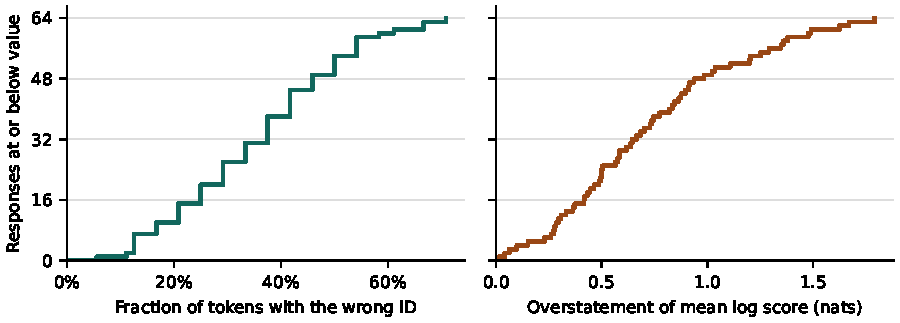
\includegraphics[width=.96\linewidth]{figures/prompt-results.pdf}
\caption{Empirical cumulative counts across the same 64 public prompts. The left panel counts responses by their fraction of misidentified positions. The right panel counts responses by the increase in the mean log score read from the original Inspect conversion. The repaired arm has zero error in both panels.}
\label{fig:prompt}
\end{figure}


A second consumer provided a decision-level contrast. We ran the released DeepEval 4.3.4 \texttt{GEval.measure} entry point~\cite{gevalpkg}, using its score-span search, candidate weighting and default 0.5 threshold. Each of 12 fixed questions had three answer variants. For each of the 36 judge requests we held the generated response fixed and corrected only its metadata. The judge was the same 135M checkpoint. The original formatter misidentified 222/1,205 positions. In 18 cases both arms produced a valid grade, always zero, and gave identical scores and decisions. In the other 18, both arms failed before returning a decision. This panel demonstrates a real consumer whose observed decisions were insensitive; its poor grade discrimination limits what it says about a capable judge.

\subsection{Choosing one answer from four}
One practical use of the mean selected-token log probability is to rank multiple answers~\cite{bestofapi}. To measure whether a change in ranking affects correctness, we selected all ARC-Easy test questions with four options labeled A through D in that order and an answer key among them~\cite{arc}. Of 2,376 test items, 2,268 qualified. Before generating, we selected the first 160 hash-ranked IDs for a pilot. Each received four unrestricted SmolLM2 chat responses at temperature 0.8, with a 12-token cap and fixed distinct seeds. Both ranking rules scored the same responses over identical positions, including an emitted stop token. The rule chose the highest mean, breaking exact ties by draw index. A leading stand-alone answer letter was compared to the external key; other responses were scored incorrect. In the pilot 65/160 winners changed text. Native ranking answered 53 questions correctly versus 48 with the reported scores (15 versus 10 correct in only one arm).

After observing the pilot we froze a confirmation on all 2,108 remaining eligible questions. On these disjoint inputs, \textbf{846 of 2,108} selected texts (40.1\%) changed; 673 parsed outcomes (A through D or invalid) differed. The first draw answered 435 questions correctly, reported-score ranking answered 446, and native-score ranking answered 470. Of the discordant questions, 163 favored native scores and 139 favored the reported scores. The paired difference of $+1.14$ percentage points has a question-bootstrap interval of $[-0.47,2.80]$ and a two-sided exact paired $p=0.186$. The observed choices changed frequently, yet their changes in correctness ran in both directions. These counts cover the eligible census under the prescribed seeds; resampling describes sensitivity to question composition.

The result extends beyond equal-score ties or invalid answers. Among 1,306 questions with a unique best score in both arms, 511 selected different draws. Among 1,939 questions where both selected texts parsed, 146 were correct only under native ranking and 133 only under wire ranking. Overall, 1,095/8,432 draws failed the answer parser, including two empty replies generated by an immediate stop token. Both remained in the analysis. The parser scores the leading letter. In one photosynthesis item, two draws began with the correct letter B but described mechanical energy. Two other draws paired a letter with its listed option, A with electrical and B with light. The reported scores chose A and the native scores chose the latter B. In a post-hoc check we counted a letter as wrong if the rest of the answer uniquely reproduced a different complete option. This caught 601 explicit contradictions in 8,432 draws and left 447 versus 417 correct selections (157 versus 127 discordances, $p=0.085$). Partial or paraphrased explanations remain outside this check.

A second analysis recomputed the means as exact fractions of the published score values. Across all 24 shared priorities for breaking ties, the number of changed texts ranged from 834 to 866 and the two-sided accuracy test had $p\geq0.169$. On 784 questions the sets of best texts were disjoint across arms, irrespective of tie resolution. On 627, even the sets of parsed outcomes were disjoint. Post-hoc text-only controls selected the first parseable answer or the most frequent parsed letter; they answered 501 and 495 questions correctly, respectively. Reliable probability reporting matters to consumers that rely on it. These counts provide no basis for choosing mean generation probability as the best question-answering rule.

\paragraph{Checkpoint transfer on the identical questions.}
Before any inference with the larger checkpoint, we fixed the same 160 pilot questions, prompts, four seeds and analysis for four-bit Qwen2.5-1.5B-Instruct on MLX-LM 0.32.2~\cite{qwenarc}. Of 1,927 sampled positions, 268 reported the wrong ID and 266 the wrong score. Changing which scores ranked the four answers changed 49/160 selected texts but only five parsed outcomes. Just three questions changed correctness: native ranking answered 136/160 correctly, wire ranking 137/160 (one native-only and two wire-only successes). The first draw also answered 136 correctly. Exact ties for best score occurred on 132 questions for native scores and 108 for wire scores. On these same questions, the smaller checkpoint changed 65 selected texts and 51 parsed answers. The two models therefore share the serialization fault, while the extent to which different texts also express different answers varies substantially.

\subsection{Fixed-trace intervention on a real optimizer}
The preceding experiments measure how completed responses are scored and selected. To isolate what would happen if a learner trusted that output, we use separate archived trajectories with an active learning signal. This experiment deliberately constrains the action space to the single-token answers A and B. Three seed-specific traces each contain 32 groups of four sampled answers to fixed labeled prompts. A keyed MLX service generated the answers. For every row the original HTTP body, native sampled token and model scores, and the learner record were linked. We preserve generation, row order, version checks, and the original group admission mask. Each arm starts from the same checkpoint. No arm resamples after parameters diverge.

For a group of four, let $A_i$ be its centered correctness reward divided by its population standard deviation plus $10^{-8}$. Let $m_i$ be the original admission indicator and $r_i$ the ratio of the current selected action probability to its recorded old probability. The loss is the negative of
\[
 \tfrac14\sum_i m_i\min\!\left(r_i A_i,\ \operatorname{clip}(r_i,0.8,1.2) A_i\right).
\]
We recompute the current two-action distribution at each optimizer step. Both candidate scores were recorded at generation time, so each old log probability uses the same two-action log normalizer. We run SGD with step size 0.05 on the 576 parameters of the final normalization layer, keeping the rest of the 135M checkpoint fixed. This group-relative, clipped objective follows established constructions~\cite{ppo,grpo}. An effective step is an observed change to the trainable parameters; nonzero derivatives on individual rows can cancel.

We use the original sampled action, its own probability, and the text-derived reward as the reference. The second arm changes only the old score to the outer value. The third changes both the action used in the loss and its old score, retaining the original text reward. The fourth also recomputes correctness and group advantages from the reported action. The last three arms represent specific consumer choices. The 64-item held-out task is shared across seeds and arms.

\begin{table}[htbp]
\centering
\caption{Fixed-trace intervention. Each triple lists seeds 17, 41, 73 in that order. There are 32 candidate group steps per seed and 64 held-out prompts. Parameter distances are measured from the corresponding reference endpoint.}
\label{tab:train}
\begin{tabular}{@{}lrrr@{}}\toprule
Fields trusted & Effective steps & Parameter distance ($L_2$) & Correct /64\\\midrule
Emitted action and score, text reward & 16 / 16 / 16 & 0 / 0 / 0 & 31 / 31 / 31\\
Outer old score only & 16 / 16 / 16 & .008 / .026 / .021 & 31 / 32 / 31\\
Outer action and score, text reward & 3 / 2 / 0 & .193 / .157 / .173 & 36 / 36 / 36\\
Outer action, score, and reward basis & 0 / 0 / 0 & .234 / .175 / .173 & 36 / 36 / 36\\\bottomrule
\end{tabular}
\end{table}

The outer action disagreed with the sampled action on 53, 53, and 51 of the 128 rows in the three traces. The reference reproduced the original per-group update records and exact final parameter hash for each seed. Substituting the old score alone left the number of effective steps unchanged, yet all three endpoint hashes changed (Table~\ref{tab:train}). Assigning the text reward to the reported action reduced effective steps to three, two and zero. For seed 73, this arm had 64 nonzero row-level log-probability derivatives and zero effective group steps. Opposing credit on the same reported action can cancel in parameter space. Scoring and training the reported action yielded zero effective steps in every trace.

One group illustrates what a test at the reward interface would see. In the first consumed group for seed 17 the emitted answers were A, B, A, A. The gold answer was B. The reference, score-only, and outer-action/text-reward arms received the same vector $(0,1,0,0)$, and all four answers passed the gate in all three arms. Only the second position was misidentified. Starting from identical weights, substituting its old score changed its log-probability derivative from $-0.43045$ to $-0.34917$ and the norm of the parameter step from 0.03891 to 0.03485. Training the reported action while retaining the text reward produced a parameter step of zero. No inspection confined to the reward vector or the admission mask could distinguish these three outcomes. The per-row derivative and parameter step supply different evidence even within one group.

The initial model already answered 36/64 held-out prompts correctly, compared with 31/64 after reference training. These data establish that incorrect metadata can alter the numerical update with the examples and admission decisions held fixed. They do not establish that correction increases task accuracy or that an existing production learner consumes these fields this way. The evaluation result above does establish propagation in a named, unmodified software path.

\subsection{When the learner collects fresh actions after each update}
The fixed trajectories isolate the first affected update but cannot measure how changed policies collect future examples. We therefore ran a synchronous online intervention. A frozen SmolLM2 backbone fed a trainable linear residual head over two legal next-token actions. Each arm sampled its own actions from its current head. Within a seed, arms shared training prompts and random uniforms. Each of 128 rounds sampled four actions per prompt for 16 prompts; binary correctness determined group-relative advantages. The reference used the actual action's old score. Each arm used its own sampled action and the reward for that draw, so subsequent actions could diverge after the first update. The fault arm took only the old score from the candidate-enabled MLX-LM 0.32.2 serializer at width one. A third arm recomputed the selected score from the collection-time snapshot. The study calls the released serializer on locally constructed policy outputs and uses a local clipped optimizer. It does not couple an external training library to the HTTP server.

We first ran 12 paired seeds in each combination of two tasks and two temperatures. Each task had 384 held-out examples. SST-2~\cite{sst} used separate train and validation splits with exact duplicates removed; number comparison used disjoint training and evaluation ranges. We use the probability allocated to the correct action as expected accuracy for one sampled answer; greedy accuracy counts the argmax. At temperatures one and two, respectively, the fault changed mean held-out probability of a correct action by $-2.84$ and $+0.08$ percentage points on SST-2 and $-2.81$ and $-1.74$ on number comparison. All four seed-bootstrap intervals included zero. In every one of the 48 comparisons, some held-out greedy decisions changed. This establishes sensitivity of individual predictions across the four conditions. It leaves their average effects uncertain.

\begin{figure}[tbp]
\centering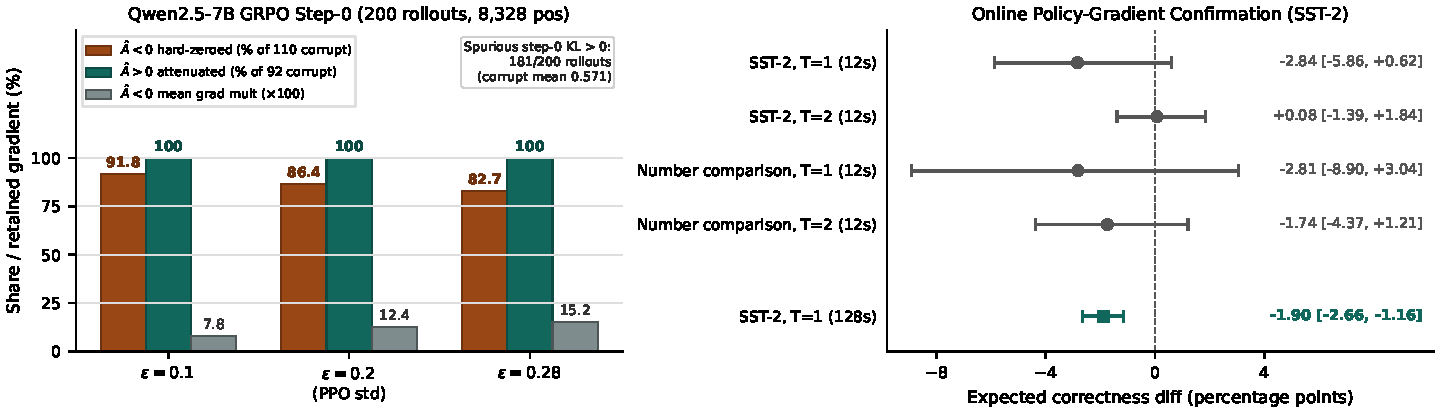
\includegraphics[width=.95\linewidth]{figures/learning.pdf}
\caption{Mean paired change in held-out probability of a correct action when training with the reported old score. Bars show 95\% bootstrap intervals across training seeds with the held-out items fixed. The bottom row uses 128 new seeds on the same split, analyzed independently of the first four rows.}
\label{fig:online}
\end{figure}

We then froze a separate confirmation restricted to the original primary condition, SST-2 at temperature one. We used the same training and validation items with 128 new training seeds and analyzed this batch separately. The reference and fault arms increased mean held-out probability of a correct response from 49.91\% at initialization to 72.15\% and 70.25\%. The paired fault effect (Fig.~\ref{fig:online}) was $-1.90$ percentage points (95\% seed-bootstrap interval $[-2.66,-1.16]$). Independently resampling paired seeds and paired held-out items within each true class gave $[-2.81,-1.02]$. Greedy accuracy was 73.22\% versus 71.03\%, a $-2.19$ point effect (crossed interval $[-3.28,-1.12]$). Across all 128 confirmation seeds, recomputing the old score from the pinned collection snapshot reproduced the reference bitwise. These intervals condition on the chosen training data, model and optimizer. The result identifies a learning consequence for one restricted policy and task.

\subsection{Does the mechanism reach the decoder itself?}
We used a new task in which two tokens classify two SST-2 reviews in order. Each token conditions on the previous one and chooses A or B. The optimizer now updates 2,433,024 original query and feed-forward down-projection weights in SmolLM2's final two decoder blocks. The frozen prefix is cached. At initialization and after a first update we checked both continuations against direct full-model forwards, with a maximum discrepancy of $1.31\times10^{-5}$ nats in the tested cells. The experiment runs the released formatter in process on the two allowed scores. The consumer retains the actual sampled actions and their reward while changing the source of the old score. A third arm recomputes the score from the original collection policy. Eight seeds each train for 32 rounds with common prompts and random draws, then evaluate on 96 held-out review pairs.

All eight pairs started with the same actions and rewards. At the first update the substitution changed 129 token denominators attached to nonzero advantages and the trained weights diverged in all eight seed pairs. Subsequent sampling differed at 2,756/15,872 paired token positions. Recomputed and reference agreed in every saved trajectory array and every recorded hash of the trainable parameters. Held-out expected exact reward rose from 25.08\% to 25.32\% under reference and 25.51\% under substitution. Neither the reference gain (+0.24 points) nor the teacher-forced control (+0.42) reached the prespecified three-point learning criterion.

We then screened two longer schedules. Both trained on the original 256 pairs and were evaluated on 128 disjoint calibration pairs drawn from the official training split. Configuration A increased the number of rounds from 32 to 128, the batch from four to six prompts and the Adam learning rate from $10^{-4}$ to $3\times10^{-4}$. Configuration B also trained untied copies of the two action readout rows while keeping the input embeddings frozen. The teacher gained 2.88 and 3.20 points on 128 calibration pairs, respectively. The correctly scored online policies changed by $-0.16$ and $-0.07$ points (two seeds per setting). Each ended with the same greedy answer pair for all 128 prompts within a run. Neither configuration qualified for the prespecified independent fault comparison. We stopped with its 160 confirmation pairs unused. The decoder experiments establish a causal change to the updates and later actions. The performance loss in Figure~\ref{fig:online} applies to the separate learning-active, single-action sentiment policy.

\section{Related work}
\paragraph{Testing stochastic systems.}
A test oracle determines whether an observed execution satisfies a specified property~\cite{barr}. Metamorphic testing derives a relation between executions whose complete expected outputs are difficult to specify~\cite{segura}. Our width comparison is an instance of that method. Its application here requires specifying which consequence of a random draw must remain invariant, which score stage is being compared, and whether one is comparing the same draw. The second invocation of the native serializer supplies a local counterfactual even when two requests would sample different text. The separate forward pass in the llama.cpp test can additionally check the value of a score without reusing a previously formatted probability.

\paragraph{Token and probability failures in serving.}
Kim's MURPHY study is a direct predecessor~\cite{murphy}. It checks record counts and per-token decoded bytes in native and chat interfaces under both transport modes and reports a buffering error in llama.cpp. It leaves the numeric accuracy of the probability values open. Its count and byte checks explain the three missing probability rows we observe on the independent implementation. MLX preserves row counts and the final transcript while substituting a different vocabulary entry within a row. We test this substitution by toggling an informational option on the same emission, then measure how much can be detected and recovered from an unchanged response. Other public reports document collisions when a completion map uses decoded strings as keys, and default-valued probabilities in speculative decoding~\cite{vllmreport,llamareport}. Such failures motivate explicit checks for token identity, row coverage, and score stage. They also preclude any broad claim that silent probability defects in servers were previously unknown.

Firestone et al.~\cite{utf8plumbing} characterized failures from decoding byte fragments separately and traced related buffering logic across serving engines. An earlier Ollama issue reported the specific symptom of replacement-character bytes in token-probability metadata~\cite{ollamabytes}. We credit this prior observation. Our cross-engine experiments distinguish a missing probability row from a present row with damaged bytes, and from an aligned row assigned to a different sampled token. Only the last mechanism explains the MLX probability shifts measured here.

Karvonen et al.\ synchronize seeds with a trusted inference implementation to verify a stochastic model under numerical nondeterminism~\cite{difr}. Their method compares the inference itself to a reference. Our same-event test accepts the actual draw and checks how it is reported. The oMLX chat implementation also gathers chosen and alternative log probabilities~\cite{omlx}. INDRA's shipped greedy restriction and its archived probe are evidence of real use~\cite{indra}. We recomputed the published label-margin analysis on 5,371 records covering 1,689 statement identifiers. The archive retains the two label scores and the verdict, without a native sampled-pair trace. It therefore supplies no estimate of historical decisions changed by this defect. Wang et al.\ showed that first-token probability rankings can disagree with a model's textual answer even under a correct reporting interface~\cite{firsttoken}. Our answer comparisons keep all four generated responses fixed while changing which observed scores rank them.

\paragraph{Using probabilities as measurements.}
Chauvin et al.\ use the variability of log probabilities to track API behavior over time~\cite{monitor}. Their target is temporal model consistency. Our intervention holds the sampling event fixed and changes its representation. It therefore tests a premise of measurements that use token probabilities as observations of generated text. In reinforcement learning, clipped policy ratios and group-relative credit provide established reasons why an action's identity and old probability matter~\cite{ppo,grpo}. Chen studied how ambiguous verifier outcomes traverse an RLVR reward pipeline~\cite{rewardfail}. Here a verifier can return the intended reward while the learner computes the policy ratio with another action's old probability. The two studies address distinct failure sites and use distinct experimental units. None of the verifier cases is counted as evidence for the serving fault.

\section{Implications and limits}
A reusable server regression needs very little generated text. Capture a real position where the decoder selected an ID other than the first candidate, serialize it with the list present and absent, and demand the same selected pair. Include a draw outside the list to discriminate a full fix from a lookup that succeeds only when the ID is already among the alternatives. A pair of equal scores for different IDs checks an additional failure mode that comparing probabilities alone misses. These tests specify no particular answer to the prompt. A renderer that buffers a character needs a separate check on how many underlying token positions have records. The measured engines pass different subsets of these checks, and their candidate-list contracts differ.

The practical remedy depends on when the user intervenes. For future requests that need only selected scores, the candidate-free MLX branch already exposes them. For users that also need alternatives, the tested source patch retains both. For old packets with no model access, Table~\ref{tab:recovery} quantifies the tradeoff between empirical recovery and abstention. Re-querying can recover more rankings on a compatible live system, but exact score recovery can depend on prior requests and prompt cache state.

The three live engines share some prompts and model lineage. The Qwen holdouts also change the architecture and tokenizer. The vLLM and SGLang checks exercise their real response builders on controlled inputs. Only the mistral.rs crossover directly compares transport modes. The MLX observer tests agreement with the raw score leaving the generator. An upstream defect shared with that observation can escape it. The llama.cpp reference uses another forward pass with shared model kernels. Thirty-six long responses establish occurrence beyond early decoding on one checkpoint and temperature. The seven FLORES strata deliberately exercise byte handling; they do not weight scripts by production frequency.

The ARC comparison covers the eligible test questions under prescribed seeds, prompts, parser and confidence rule. Free-form judging and PPO outcomes have different eligibility and sensitivity conditions. The training interventions use a restricted action space with a chosen consumer and one training split per task. Neither public software usage nor our local rates measure how often a deployed system takes a wrong decision. That requires independently sampled deployment requests joined to the original emitted scores, the reported data and the actual decision. More draws from our existing workloads cannot supply that sampling frame.

\section{Conclusion}
Testing a formatter against the emission that it received exposed a sampled-token substitution even when the generated text and row count looked correct. A source patch restored the sampled fields while preserving the alternatives. After serialization, the options narrow. Two different native rankings can produce the same response objects, and a seeded repeat can reproduce an answer without reproducing its scores. Downstream, this defect changed hundreds of selected answer texts and altered real optimizer updates. Its effect on correctness depended on the consumer and workload. These distinctions let a serving team test a specific contract, choose a remedy for the information it retains, and measure consequences without inferring them from field mismatches alone.

\section*{Data Availability}
The TokenReceipt repository provides selected replication materials at \url{https://github.com/feiiiiii5/tokenreceipt}. The complete research archive prepared for anonymous review contains the saved observations, pinned sources, protocols, and executable checks for the comparisons reported here. It includes the source patch for MLX-LM 0.32.2, the HTTP regression panel, the normalized counterexample, and separate instructions for offline recomputation and live reruns. The archive includes the 541 IFEval keys, their frozen ranking digests, and the hashes of the 64 selected prompts. The digests use SHA-256 over the prefix \texttt{rewardfail-raw-chat-v1/} followed by the decimal key. Live MLX inference requires a compatible Apple runtime and the pinned public checkpoint.
\bibliographystyle{unsrtnat}
\bibliography{references}
\end{document}
